%Bạn không cần phải sử dụng minipage như mình mà có thể dùng rời ra.
\begin{tcolorbox}
\begin{bt}
Cho khối chóp $S.ABCD$ có đáy $ABCD$ là hình thoi cạnh bằng $2$, $\widehat{ABC} = 120^\circ$, $SD = SA$. Mặt phẳng $(SAD)$ vuông góc với đáy và cạnh bên $SA$ tạo với mặt phẳng đáy một góc $60^\circ$. Thể tích khối chóp $S.ABCD$ bằng bao nhiêu?
\end{bt}
\begin{sol}\textcolor{white}{.}\\
\begin{minipage}{0.65\textwidth}
$SA$ tạo với mặt phẳng đáy một góc $60^{\circ}$, nghĩa là $\widehat{SAH}=60^{\circ}$. Ta suy ra $SH=AH\cdot \tan{60^{\circ}}=\sqrt{3}$. Vì $\widehat{ABC}=120^{\circ}$ nên $AC=2\sqrt{3}$ và $DB=2$ nên diện tích đáy $S_{ABCD}=\dfrac{1}{2}.2\sqrt{3}.2=2\sqrt{3}$. Do đó, thể tích khối chóp $S.ABCD$ là: $V=\dfrac{1}{3}.\sqrt{3}.2\sqrt{3}=2.$
\end{minipage}
\begin{minipage}{0.4\textwidth}
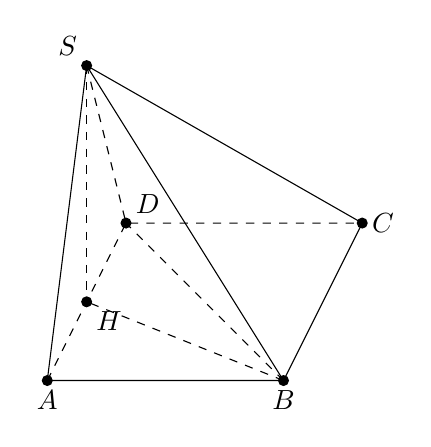
\begin{tikzpicture}
\draw[color=black](0,0)node[below]{$A$}--(3,0)node[below]{$B$}--(4,2)node[right]{$C$};
\draw[color=black](0.5,4)--(0,0);
\draw[color=black](0.5,4)--(3,0);
\draw[color=black](0.5,4)node[above left]{$S$}--(4,2);
% \draw[color=black](2.5,3)--(2,-2.5);
\draw[dashed](0,0)--(0.5,1)node[below right]{$H$}--(1,2)node[above right]{$D$};
\draw[dashed](0.5,4)--(1,2)--(4,2);
\draw[dashed](0.5,4)--(0.5,1);
\draw[dashed](3,0)--(0.5,1);
\draw[dashed](3,0)--(1,2);
\fill (0,0) circle (2pt); 
\fill (3,0) circle (2pt);
\fill (4,2) circle (2pt);
\fill (1,2) circle (2pt);
\fill (0.5,1) circle (2pt);
\fill (0.5,4) circle (2pt);
\end{tikzpicture}
\end{minipage}
\end{sol}
\end{tcolorbox}
